% !TeX spellcheck = en_GB
\chapter{The Alexandrov Reflection Method}

\section{Geometry of immersed hypersurfaces}


The study of immersed hypersurfaces is a fundamental topic in differential geometry, and is especially important in the field of geometric analysis. An immersed hypersurface $X: M^n \rightarrow \overline{M}^{n+1}$ is a submanifold of a higher-dimensional space that is embedded in that space in such a way that the submanifold has the same dimension as the space in which it is embedded minus one. In other words, it is a submanifold of codimension one. We will always assume the embedding to be smooth. The most common case is $\overline{M}^{n+1}=\R^{n+1}$, usually extensively studied in undergraduate courses when $n=2$. We will be assuming that the embedding is also isometric, i.e. the metric $g$ on $M^n$ is the one induced by $(\overline{M}^{n+1}, \overline{g})$. 

\begin{figure}
	\centering
	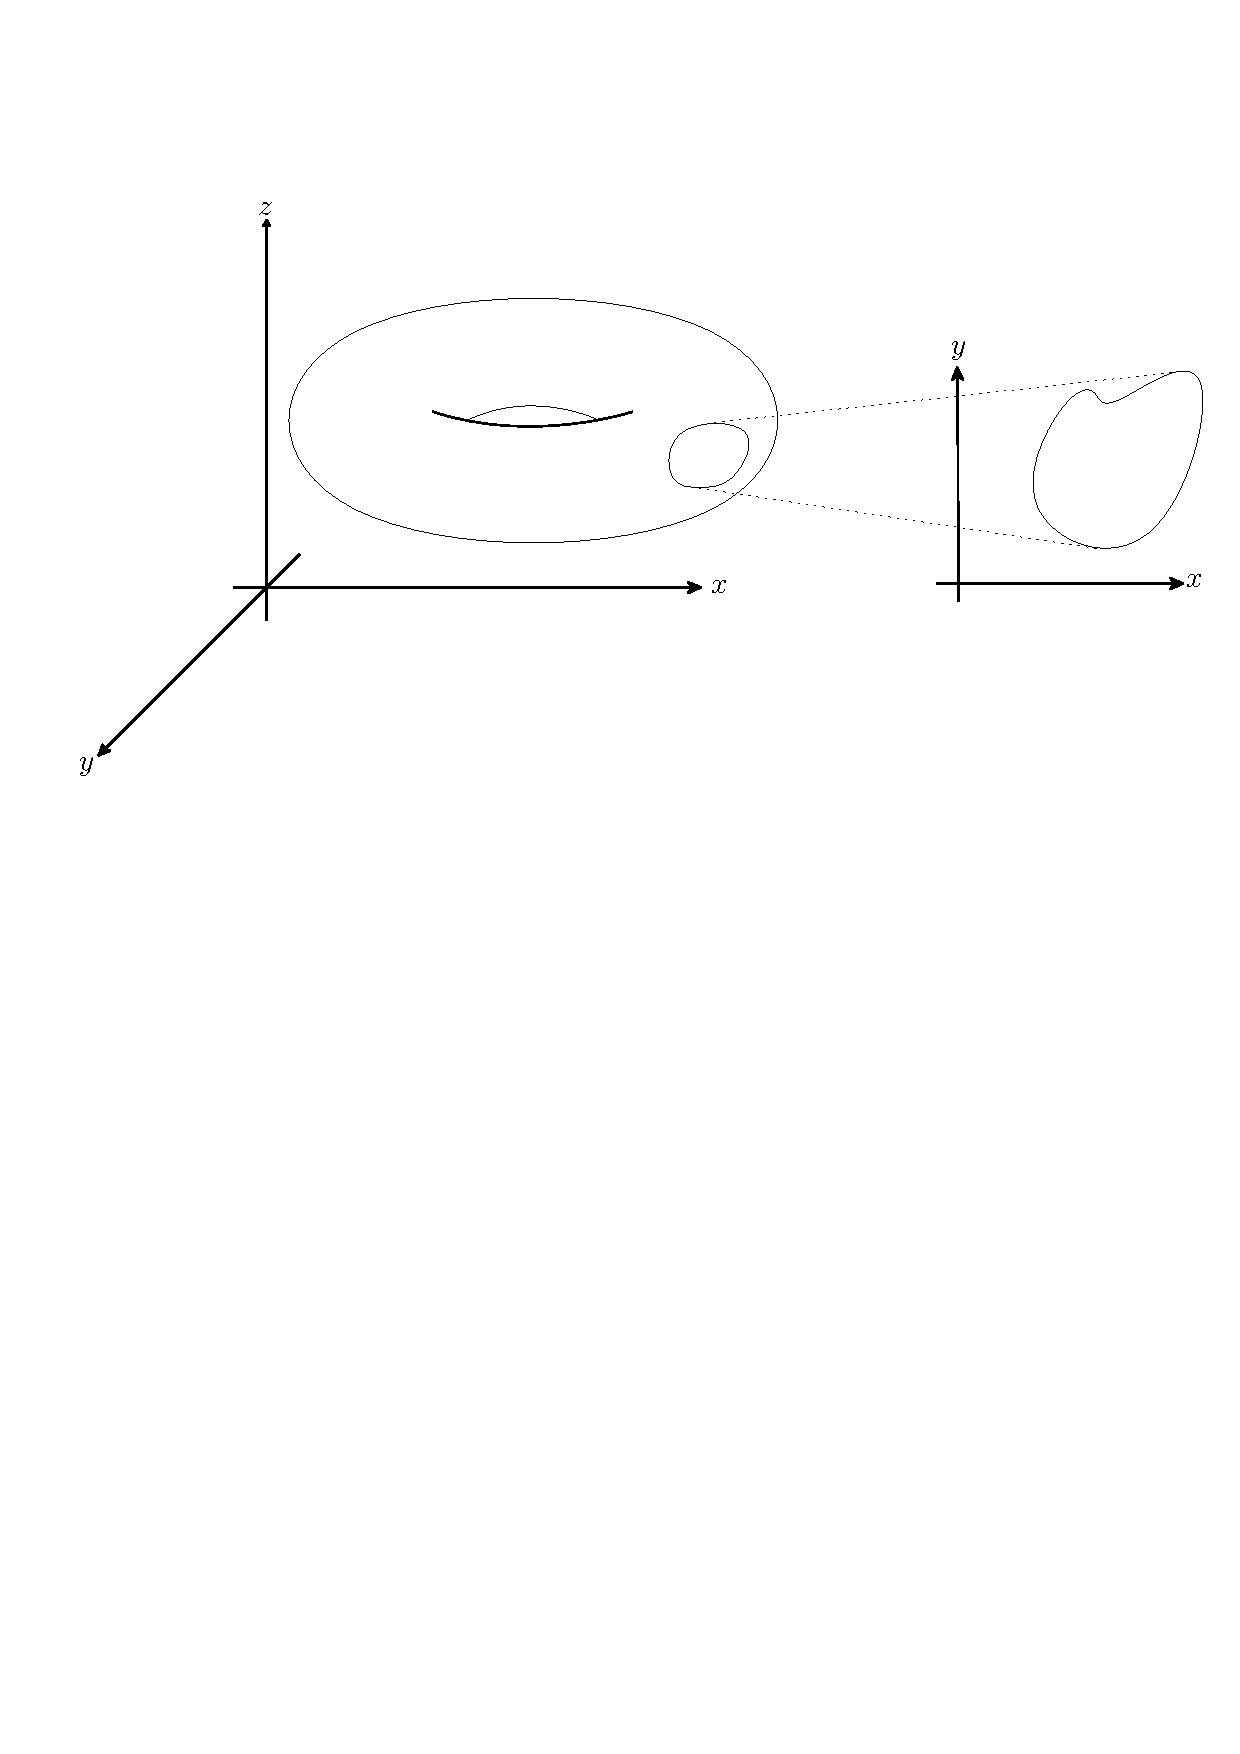
\includegraphics[width=0.713\textwidth]{figures/embedded_manifold.pdf}
	\caption{A (hyper)surface immersed in $\R^3$}
\end{figure}

Symbols referring to $(\overline{M}^{n+1}, \overline{g})$ will have a line on top, otherwise the symbol will refer to $(M^{n}, g)$.


The pullback of the tangent bundle of $\overline{M}^{n+1}$ to
$M^{n}$ is a smooth vector bundle on $M^{n}$:
\begin{align*}
	X^{*}T\overline{M}^{n+1}=T\overline{M}^{n+1}|_{M^n}= \amalg_{p \in M^n} T_p\overline{M}^{n+1}
\end{align*} 

\begin{figure}
	\centering
	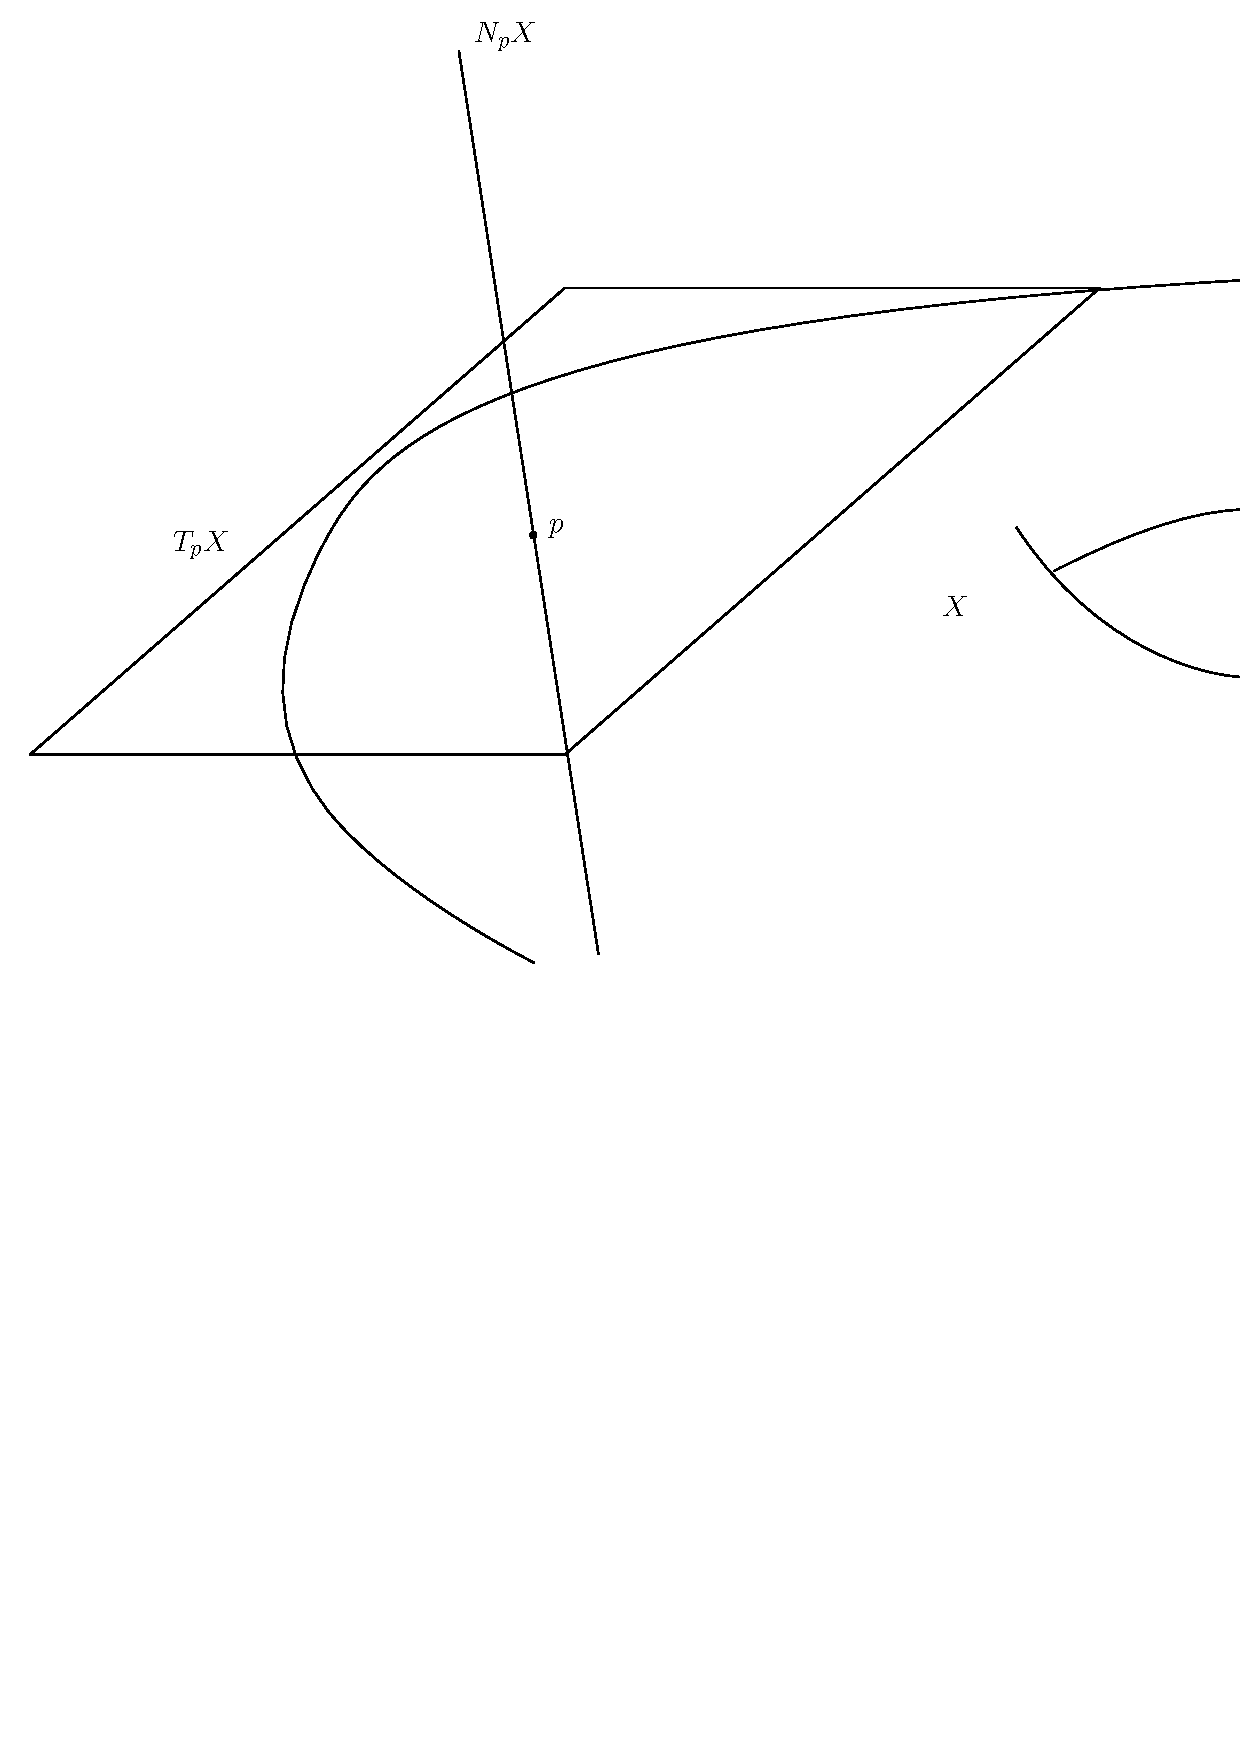
\includegraphics[width=\textwidth]{figures/tangent_and_normal_bundles}
	\caption{The tangent and the normal bundle at a point $p$}
\end{figure}


One of the most important concepts in the geometry of immersed hypersurfaces is the concept of a normal vector field. The normal vector field $\nu$ is a section of the pullback vector bundle $X^* TM^{n+1}$ on the manifold $M^n$ that is perpendicular to the tangent space of $M^n$ at each point. At each point $p$:
\begin{align*}
	T_p\overline{M}^{n+1}=T_pM^{n}\oplus N_pM^{n}
\end{align*} 
where $N_pM^{n}$ is the normal vector bundle generated by the normal vector. This also allows us to define the tangent and normal projection on $T\overline{M}^{n+1}|_{M^n}$ by taking the two respective components. 

Clearly, taking $\overline{\nabla}$ to be the Levi-Civita connection on $(\overline{M}^{n+1}, \overline{g})$, we can decompose it as:
\begin{align*}
	\overline{\nabla}_v w = (\overline{\nabla}_v w )^\top +  (\overline{\nabla}_v w )^\bot
\end{align*} 

\begin{defin}
	The {\em second fundamental form} is then defined as: 
	\begin{align*}
	 	\mathrm{I\!I} (v, w) =  (\overline{\nabla}_v w )^\bot 	
	\end{align*} 
\end{defin}
It is a bilinear symmetric tensor because $TM^n$ is involutive in $T\overline{M}^{n+1}$ and depends only on the local value of $v$ and $w$ by symmetry. we can therefore write it as
\begin{align*}
	\mathrm{I\!I} (v, w) = -(h_{ij}v^iw^j)\nu
\end{align*} 
for some matrix $A(p)=\{h_{ij}\}$. we can define the principal curvatures of the hypersurface, as the eigenvalues of this matrix.

It is also possible to check that $(\overline{\nabla}_v w )^\top$ satisfies the definition the Levi-Civita connection on $(M^n, g)$, therefore, from its uniqueness:
\begin{align*}
	\nabla_v w &=  (\overline{\nabla}_v w )^\top	\\
	\overline{\nabla}_v w &= \nabla_v w  + \mathrm{I\!I} (v, w) 
\end{align*} 
where $\nabla$ is the Levi-Civita connection on $(M^n, g)$. This result is known as the {\em Gauss Formula}. It has to be noted however that we are implicitly considering tangent vectors that are not in the same space. Indeed, making that more explicit, the formula should be:
\begin{align*}
	\overline{\nabla}_{X_*v} X_* w &= X_* (\nabla_v w)  + \mathrm{I\!I} (v, w) 
\end{align*}

\begin{proposition}
	\textbf{\em (The Weingarten Equation)} If $v, w \in TM^n$ and $\nu \in NM^n$, if one considers the corresponding derivations in $T\overline{M}^{n+1}$ the following equation holds:
	\begin{align*}
			\left\langle \overline{\nabla}_v \nu, w \right\rangle_{\overline{g}} = - \left\langle \nu, \mathrm{I\!I} (v, w) \right\rangle_{\overline{g}}
	\end{align*}
\end{proposition}
\begin{proof}
	As $\left\langle \nu, w \right\rangle_{\overline{g}}\equiv 0$ on $M$, 
	\begin{align*}
		0&=v\left\langle \nu, w \right\rangle_{\overline{g}}\\
		&=\left\langle  \overline{\nabla}_v \nu, w \right\rangle_{\overline{g}} + \left\langle  \nu, \overline{\nabla}_v w \right\rangle_{\overline{g}}\\
		&=\left\langle \overline{\nabla}_v \nu, w \right\rangle_{\overline{g}} + \left\langle \nu, \mathrm{I\!I} (v, w) \right\rangle_{\overline{g}}
	\end{align*}
	applying the Gauss Formula and the fact that $\nabla_v w \in TM^n$ in the last step
\end{proof}
It is also usual to define the associated Weingarten map, which is the linear map between sections of $M$  $s:\Gamma(M)\rightarrow\Gamma(M)$ satisfying:
\begin{align*}
	\left\langle s(v), w \right\rangle_{g} = \left\langle \nu, \mathrm{I\!I} (v, w) \right\rangle_{\overline{g}}
\end{align*}
the linear map $s$ is also known as the {\em shape operator of $M$}. 

Combining this with the formula above, taking into account that it holds for a generic $w \in TM$:
\begin{align*}
	s(v) = -(\overline{\nabla}_v \nu)^\top
\end{align*}


We are going to use these equations in local coordinates, in the form shown below. 
\begin{proposition}
	The above equations in local coordinates are equivalent to the following equations:
	\begin{align}
		\label{Weingarten1} \frac{\partial^2 X^\alpha}{\partial x^i \partial x^j} - \Gamma^k_{ij}\frac{\partial X^\alpha}{\partial x^k}+\overline{\Gamma}^\alpha_{\beta \delta}\frac{\partial X^\beta}{\partial x^i}\frac{\partial X^\delta}{\partial x^k}=-h_{ij}\nu^\alpha \\
		\label{Weingarten2} \frac{\partial \nu^\alpha}{\partial x^i}+\overline{\Gamma}^\alpha_{\beta \delta}\frac{\partial X^\beta}{\partial x^i} \nu^\delta = h_{ij}g^{jl}\frac{\partial X^\alpha}{\partial x^l}
	\end{align} 
	where $\nu$ is the normal unit vector at the point and $A=\{h_{ij}\}$ is the second fundamental form, thus $h_{ij}= \left\langle  \nu, \overline{\nabla}_{\overline{\partial_i}} \overline{\partial_j} \right\rangle_{\overline{g}} $
\end{proposition}
\begin{proof}
	For any connection $\nabla_\cdot$ and any derivations $v=v^i \partial_i$ and $w=w^j \partial_j$:
	\begin{align*}
		\nabla_{v} w = \nabla_{(v^i \partial_i)} (w^j \partial_j) = v(w^k)\partial_k + (v^i w^j \Gamma^{k}_{ij})\partial_k
	\end{align*}
	Let $\partial_1, \dots \partial_n$ be a basis of $TM^n$ at a point, and let $\overline{\partial_i} = X_*\partial_i$, $\overline{\partial_{n+1}}=\nu$.
	Let's consider the Gauss Formula for two generic $\partial_i$, $\partial_j$, using roman letters for indices varying between $1$ and $n$ and greek letters for indices varying between $1$ and $n+1$, and $\delta^{ij}$ the Kronecker delta:
	\begin{align*}
		\overline{\nabla}_{X_*\partial_i} X_* \partial_j &= X_* (\nabla_{\partial_i} \partial_j)  + \mathrm{I\!I} (\partial_i, \partial_j) \\
		(\overline{\partial_i}(X_*\partial_j)^\alpha) \partial_\alpha + ((X_*\partial_i)^\beta (X_*\partial_j)^\delta \overline{ \Gamma}^{\alpha}_{\beta \delta})\partial_\alpha &= X_* (\cancel{(\partial_i \delta^{jk})\partial_k} +  \delta^{ij}\Gamma^{k}_{ij}\partial_k)  - h_{ij}\nu^\alpha \overline{\partial_\alpha}\\
		(\overline{\partial_i}(X_*\partial_j)^\alpha) \partial_\alpha + ((X_*\partial_i)^\beta (X_*\partial_j)^\delta\overline{ \Gamma}^{\alpha}_{\beta\delta})\partial_\alpha &= X_* (\Gamma^{k}_{ij}\partial_k)  - h_{ij}\nu^\alpha \overline{\partial_\alpha}\\
		\frac{\partial^2 X^\alpha}{\partial x^i \partial x^j} +\overline{\Gamma}^\alpha_{\beta \delta}\frac{\partial X^\beta}{\partial x^i}\frac{\partial X^\delta}{\partial x^k}&=\Gamma^k_{ij}\frac{\partial X^\alpha}{\partial x^k}-h_{ij}\nu^\alpha
	\end{align*}
	Which is the formula (\ref{Weingarten1}). 
	To get the second formula, first note that $s(v) = -(\overline{\nabla}_v \nu)^\top$. We then compute $-\langle s(\partial_i), \overline{\partial_\alpha}\rangle_{\overline{g}}$:
	\begin{align*}
		\left\langle\overline{\nabla}_{\overline{\partial_i}} \nu, \overline{\partial_\alpha}\right\rangle_{\overline{g}} &= -\left\langle s(\partial_i), \overline{\partial_\alpha}\right\rangle_{\overline{g}}\\
		\left\langle \left(\frac{\partial \nu^\alpha}{\partial x^i}+\overline{\Gamma}^\alpha_{\beta \delta}\frac{\partial X^\beta}{\partial x^i} \nu^\delta \right)\overline{\partial_\alpha}, \overline{\partial_\alpha} \right\rangle_{\overline{g}}&= h_{ij}g^{jl}\frac{\partial X^\alpha}{\partial x^l}
	\end{align*}
	leading to (\ref{Weingarten2}).
	\begin{comment}
	Similarly, taking the Weingarten Equation and the definition of $h_{ij}$:
	\begin{align*}
		h_{ij} &=\left\langle  \nu, \overline{\nabla}_{\overline{\partial_i}} \overline{\partial_j} \right\rangle_{\overline{g}} = - \left\langle  \overline{\nabla}_{\overline{\partial_i}} \nu, \overline{\partial_j} \right\rangle_{\overline{g}}\\
		&= - \left\langle \overline{\partial_i}(\nu^\alpha) \overline{\partial_{\alpha}} + ((\overline{\partial_i})^\beta \nu^\delta \Gamma^{\alpha}_{\beta\delta})\overline{\partial_\alpha}, \overline{\partial_j} \right\rangle_{\overline{g}} \\
		&= - \left\langle  (\frac{\partial \nu^\alpha}{\partial x^i}+\overline{\Gamma}^\alpha_{\beta \delta}\frac{\partial X^\beta}{\partial x^i} \nu^\delta )\overline{\partial_\alpha}, \overline{\partial_j} \right\rangle_{\overline{g}}		
	\end{align*}
	Which leads to (\ref{Weingarten2}) by applying the inverse of the metric $g^{jl}$ to both sides. 
	contenuto...
	\end{comment}
\end{proof}


% The Weingarten equations are important in the study of the local properties of immersed hypersurfaces, for example, the second kind equation relates the normal vector field to the shape operator and can be used to compute the mean curvature of the hypersurface. 

% Another important concept in the geometry of immersed hypersurfaces is the Gaussian curvature. The Gaussian curvature is a scalar valued function that describes the total curvature of the hypersurface at each point. It is defined as the product of the eigenvalues of the shape operator and it is closely related to the sectional curvature of the ambient space.

%There exist many important partial differential equations (PDEs) which stem from the study of immersed hypersurfaces, for example, the minimal surface equation, which is a PDE that describes surfaces with minimal area, can be seen as a geometric condition on the mean curvature of an immersed hypersurface. Likewise, the mean curvature flow is a geometric flow that deforms an immersed hypersurface by moving each point along the normal vector field at that point by an amount proportional to the mean curvature at that point. This flow is important in the study of geometric PDEs and is used to obtain a lot of important results in differential geometry.

% Some other important results useful for the study of PDEs on immersed manifolds are:


%The Gauss-Codazzi equations: These are a set of equations that relate the curvature of an immersed hypersurface to the curvature of the ambient space. These equations are important in the study of geometric PDEs and are used to obtain a lot of important results in differential geometry.

%The Gauss equation: This is an equation that relates the Gaussian curvature of an immersed hypersurface to the sectional curvatures of the ambient space. It is important in the study of the global properties of immersed hypersurfaces.

%The Gauss-Bonnet theorem: This is a theorem that relates the Gaussian curvature of an immersed hypersurface to the topology of the hypersurface. It is important in the study of the global properties of immersed hypersurfaces and is used to prove many important results in differential geometry.

\section{Local representation as a graph}

A well known result, Dini's Theorem\footnote{also known as Implicit Function Theorem}, states that, given a smooth function $F$ defined on an open subset of the product space $\R^n \times \R^m$, if $F(x,y) = 0$ and the partial derivative of $F$ with respect to $y$ is nonzero at a point $(x_0, y_0)$, then there exists an open neighborhood of $x_0$ in $\R^n$ and a unique smooth function $y = g(x)$ defined on that neighborhood such that $y_0$ is a regular value of $g$ and $(x, g(x))$ is a smooth solution to the equation $F(x, y) = 0$.

Consequence of the Dini's theorem is a powerful result that allows one to locally represent a submanifold of $\R^n \times \R^m$ as the graph of a smooth function. This theorem is widely used in differential geometry, geometric analysis, and many other fields of mathematics and physics. We provide a version of this theorem below:

\begin{theorem}[Local representation as a graph]
	Let $X^n$ be a submanifold $X^n\subset\R^{n+1}$ and let $x_0\in X$. Then there exists a neighbourhood of $x_0$, $U\subset X^n$, such that $U$ is the graph of a function. 
	Moreover, this function can be of the form 
	\begin{align*}
		f:\pi(U)\subset&\R^n\rightarrow U \\
		U=\{(x_0, \dots, x_n)\in \R^{n+1}&|x_0= f(x_1, ..., x_n)\}
	\end{align*}
	for any of the possible orders of the usual basis for $\R^n$, $(e_0, \dots, e_n)$, as long as $e_0\notin T_xM$, where $\pi(U)$ is the projection on the last $n$ coordinates ($(x_0, \dots, x_n) \mapsto (x_1, \dots, x_n)$). \label{localgraphclassic}
\end{theorem}

A proof of the 2D-case of the version of the theorem can be found in \cite{DoCarmo} which extends naturally to the $n$ dimensional case, with almost no changes. This immediately extends to:

\begin{cor}[Local representation as a graph on the tangent]
	Let $X^n$ be a submanifold $X^n\subset\R^{n+1}$ and let $x_0\in X$. Then there exists a neighbourhood of $x_0$ $U\subset X^n$ and a smooth function $f: T_x X^n\rightarrow \R$ such that any $x_0\in U$ can be expressed as \label{localgraphcorollary}
	\begin{align*}
		x_0= p + f(p) \nu 
	\end{align*}
	where $\nu$ is the vector normal to $T_{x_0} X^n$, for an appropriate point $p\in T_{x_0} X^n$. 
	In other words, every submanifold $X^n\subset\R^{n+1}$ is locally expressible as a graph on its tangent space. 
\end{cor}

\begin{proof}
	By rotation, we may assume $T_x X^n$ orthogonal to $e_1$. Then one can just apply the previous theorem. 
\end{proof}

We will use this later to prove Theorem \ref{localgraph}. 


\section{Some well established results from analysis}

We now introduce some well known results from analysis. The first result we introduce is the maximum principle.

The maximum principle is a classical result of mathematical analysis, and it is usually introduced in a first course on partial differential equations. It is a fundamental tool in the theory of partial differential equations. It is a statement about the behavior of solutions to certain types of PDEs and provides a method for obtaining upper and lower bounds on the solutions. The principle states that the maximum and minimum values of a solution to elliptic or parabolic PDE occur on the boundary of the domain unless the function is constant. 

The maximum principle can be used to prove the existence, uniqueness, and regularity of solutions to elliptic and parabolic PDEs. It can also be used to obtain estimates on the behavior of solutions and to study the asymptotic behavior of solutions as the domain becomes large. The principle is widely used in many fields of mathematics and physics, such as geometric analysis, mathematical physics, and fluid dynamics. One of the many versions of this well know theorem is this: 

\begin{theorem}[Maximum principle for parabolic equations]\label{maximum_principle}
	Let $\Omega$ be an open, bounded, connected set. Assume $u\in C^2_1(\Omega\times [0, T])\cap C^1(\overline{\Omega}\times [0, T])$. Suppose $u$ satisfies: 
	\begin{align}
		-\frac{\partial u}{\partial t} + \left(\sum_{i, j=1}^n a_{ij}\frac{\partial^2 }{\partial x_i\partial x_j}+\sum_{i}^n b_{i}\frac{\partial }{\partial x_i} + c\right)  u = -u_t + Lu \geq 0 \label{condition_max_principle}
	\end{align}
	where $L$ is an elliptic differential operator, i.e. there exists $\theta>0$ such that $\sum_{i,j=1}^{n} a_{ij}(x, t) \xi_i\xi_j \geq \theta |\xi |$ for all $\xi \in \R^n$ and $(x, t) \in \Omega\times[0, T]]$. Suppose also that $c\equiv 0$ in $\Omega$. Then: \begin{itemize}
		\item if $u$ attains its maximum in an interior point $(x_0, t_0)\in\Omega\times [0, T]$, then $u$ is constant in $\Omega\times [0, t_0]$.
		\item If, instead, under the same conditions, $u_t+ Lu \geq 0$ and attains its minimum in an interior point of $\Omega\times [0, T]$, then $u$ is constant in $\Omega\times [0, t_0]$
	\end{itemize}
\end{theorem}
A proof of this result can be found, for example, in \cite{Evans}. The theorem extends also to situations where the condition holds in a convex bounded connected region $R\subseteq \Omega \times [0, T]$: in that case, if $u$ attains its maximum in an interior point then $u$ has the same value at any point in $R$ that can be connected to it through a segment going in the backwards direction of time and a "horizontal" line contained in $\Omega$. This version of the theorem can be found for example in \cite{protterweinberger}: 
\begin{theorem}
	Let $u$ satisfy the uniformly parabolic differential inequality (\ref{condition_max_principle}) with $c(x)\leq 0$
	in a region $R_T =\{(x_1,x_2, \dots ,x_n ,t)\vert t\leq T\}$ where $R$ is a non-empty connected open set, and suppose that the coefficients of $L$ are bounded. Suppose that the maximum of $u$ in $R_T$ is $M$ and that it is attained at a point $(x, t)$ of $R_T$. Thus if $(y,s)$ is a point of $R$ which can be connected to $(x,t)$ by a path in $R$ consisting only of horizontal segments and upward vertical segments, then $u(y,s) = M$.\label{maxprincprotterweinberger}
\end{theorem}

Hopf's boundary point lemma is another important classical tool in the study of PDEs that provides a criterion for determining the behavior of solutions to certain types of elliptic or parabolic PDEs near the boundary of the domain. The lemma states that if one has a solutions to some kinds of partial differential inequalities, then the normal derivative of the solution at that point is strictly positive.

It is often used to obtain estimates on the behavior of solutions near the boundary, and to prove the existence and uniqueness of solutions to boundary value problems. The lemma is named after the German mathematician Eberhard Hopf, who first formulated it in the 1950s. In \cite{protterweinberger} we find the following version of the Hopf's boundary point lemma:

\begin{theorem}
	Let u be a solution to the parabolic inequality 
	\begin{align*}
		-u_t+Lu\geq 0
	\end{align*} 
	with $L$ an elliptic linear differential operator with bounded coefficients such that $c(x)\leq 0$,in a domain $E$, and let $E_t = \{(x, s) \in E | s \leq t\}$. Suppose the maximum $M$ of $u$ is attained at a point $P=(x, t)$ on the boundary $\partial E$. \\
	Assume that a sphere through $P$ can be constructed which is in $E_s$ such that
	\begin{itemize}\itemsep0em 
		\item tangent to $\partial E$ at $P$
		\item the set of point of its interior $(y, s)$ such that $s\leq t$ lies in $E_s$, 
		\item  $u < M$ in its interior.
	\end{itemize}	
	Also, suppose that the radial direction from the centre of the sphere to P is not parallel to the t-axis. \\
	Then, if $\frac{\partial}{\partial \nu}$ denotes any directional derivative in an outward direction from $E_s$ , we have
	\begin{align*}
		\frac{\partial u}{\partial \nu} > 0
	\end{align*}
	at P.\label{HopfBPL}
\end{theorem}
\begin{proof}
	Let the sphere through $P$ be $B_1$. We may construct a smaller sphere $B_2$ centred at $P$. Let now:
	\begin{align*}
		S_1 &= \partial B_1 \cap  B_2 \cap E_t, \\
		S_2 &= B_1 \cap \partial  B_2 \cap E_t, \mathrm{ and} \\
		S_3 &= B_1 \cap  B_2 \cap \partial E_t= B_1 \cap  B_2 \cap \{(x, s) \in E | s=t\}.
	\end{align*}
	The three sets satisfy $S_1\cup S_2 \cup S_3 = \partial (B_1 \cap  B_2 \cap E_t)$, we may call this region $R=B_1 \cap  B_2 \cap E_t$. Without loss of generality, potentially taking a smaller sphere $B_1$, we may assume that $u<M$ on $B_1$ except at $P$. As $R \subset B_1$, we also get  $u<M$ on $R$. 
	We may thus conclude that: 
	\begin{itemize}\itemsep0em 
		\item  $u<M$ on $R$ except at $P$
		\item  $u\leq M-\delta$ on $S_2$ for a sufficiently small $\delta>0$
		\item  $u=M$ at $P$.
	\end{itemize}	
	Now, let the centre of $B_1$ be $Q=(z, t_0)$ and let $r$ be its radius. we can now introduce the function	
	\begin{align*}
		v(y, s) = exp \left(-\alpha(s-t_0)^2-\sum_{i=1}^n\alpha(y_i-z_i)^2\right) - exp\left(-\alpha r^2\right)
	\end{align*}
	This function is such that $v(y, s)=0$ if $(y, s)\in S_1$ - including  $v(x, t)=0$, as there the first term is $e^{-\alpha r^2}$, and $v(y, s)>0$ in the interior of $B_1$.  \\
	Thus, in the region $R$, $v(y, s)\geq0$ and has a minimum point at the boundary on $(x, t)$, where  $v(x, t)=0$.
	
	We can also compute $Lv$. After some calculation, we get that 
	\begin{align*}
		Lv = 2 \alpha e^{\left(-\alpha(s-t_0)^2-\sum_{i=1}^n\alpha(y_i-z_i)^2\right)}[2\, \alpha\, (y-z&)^t A (y-z) +\\
		+&\sum_{i}^n[ b_i (y_i-z_i)+a_{i,i}]+(s-t)]
	\end{align*}
	where $A$ is the matrix of the $a_{i,j}$. In particular, one can choose an $\alpha$ large enough, so that $Lv>0$ in $R\cup \partial R$.
	
	We can thus introduce $w=u+\varepsilon v$. As both $Lu$ and $Lv$ are positive in $R$, $Lw>0$ in $R$. We can also choose $\varepsilon$ small enough so that $w<M$ on $S_2$. Also, as $v=0$ on $S_1$, $w<M$ on $S_1$ except at $P$, and $w=M$ at $P$.
	
	Therefore, we can apply the Strong Maximum Principle \ref{maxprincprotterweinberger} to the region $R$ to conclude that the maximum of $w$ in $R$ is attained at $P$. Therefore:
	\begin{align*}
		\frac{\partial w}{\partial \nu}=\frac{\partial u}{\partial \nu}+\varepsilon\frac{\partial v}{\partial \nu}\geq0
	\end{align*}
	But:
	\begin{align*}
		\frac{\partial v}{\partial \nu}=\nu \cdot n\frac{\partial v}{\partial R} = - 2\nu \cdot n \alpha Re^{-\alpha R}<0
	\end{align*}
	Where $n$ is the vector orthogonal to the sphere $S_1$. Therefore, one must have:  
	\begin{align*}
		\frac{\partial u}{\partial \nu}>0
	\end{align*}
	as we wanted.
\end{proof}
\begin{oss}\label{removecpositive}
	\em If $c(x)$ is now just bounded, we can consider, instead of $u$, $v= u e^{-\lambda t}$, thus, by change of variables 
	\begin{align*}
		-v_t+Lv-\lambda v \geq 0
	\end{align*}
	whenever $-u_t+Lu\geq 0$, and we can chose $\lambda$ large enough such that $c(x)-\lambda<0$ and thus we can remove the hypothesis $c(x)\leq0$ in both theorems when $c$ is bounded. 
\end{oss}

\section{Applying the maximum principle to non-linear PDEs}
\label{non linear pde parabolic section}
We can now introduce an important observation shown in \cite{protterweinberger} that allows us to apply the maximum principle \ref{maxprincprotterweinberger} and Hopf's boundary point lemma \ref{HopfBPL} in some non-linear settings.  Firstly, we must clarify what we mean by parabolic non-linear problem. 
\begin{defin}\label{nonlinearpde}
	A differential non-linear problem in the form 
	\begin{align}
		Lu= F\left(t, x, v, \frac{\partial v}{\partial x_i} , \frac{\partial^2 v}{\partial x_i \partial x_j}\right)-v_t = f(x, t)\label{nonlinearexample}
	\end{align} 
	given a smooth $F$ is parabolic if for any real vector $\xi$
	\begin{align*}
		\sum_{i, j=1}^n F_{ij}\xi_i\xi_j >0
	\end{align*} 
	where $F_{ij}$ are the derivatives of $F$ with respect to $\frac{\partial^2 v}{\partial x_i \partial x_j}$. 
\end{defin}
\begin{comment}
	First, let's introduce an easier example from \cite{GidasNirenberg}: 
	Suppose that $u$ solves:
	\begin{align}
		u_t-L u+f(u)=0 \label{non-linear}
	\end{align}
	For an elliptic operator $L$, and where $u_t=\frac{\partial u}{\partial t}$. We note that this differs from the usual parabolic equation because here $f$ depends from the solution $u$, potentially in non-trivial ways, making the equation non-linear. 
	If a solution exists, and $f$ is a $C^1$ function, by the theorem of the mean, at any point $x$ in the domain of $u$ we can find a function $\xi(x)$ such that
	\begin{align*}
		f'(\xi(x))&=\frac{f(u(x))-f(0)}{u(x)-0}\\
		f'(\xi(x))u&=f(u(x))-f(0)
	\end{align*} 
	If $u$ solves (\ref{non-linear}), and if $f(0)\leq0$, then 
	\begin{align*}
		u_t-L u+f(u)-f(0) &\geq 0\\
		u_t-L u+ f'(\xi(x))u&\geq 0 \\
		u_t-L u+ c(x)u&\geq 0
	\end{align*}
	Hence the function $u$ is the super-solution to a (different) linear parabolic partial differential equation and hence we can apply the maximum principle \ref{maxprincprotterweinberger} and Hopf's boundary point lemma \ref{HopfBPL} to solutions of (\ref{non-linear}) as long as the other hypothesis apply to $c(x)$. 
\end{comment}
Secondly, we remind the reader of the following generalized version of the theorem of the mean, a.k.a. Lagrange's theorem:
\begin{theorem}[Lagrange's theorem]
	Given a convex open set $U\subseteq \R^n$ and a real function $F \in C^1(U)$, and given to points $x, y$ in $U$, there exists a point $z$ in the segment connecting $x$ and $y$ such that 
	\begin{align*}
		F(y)-F(x) =\left\langle \nabla F(z), (y-x) \right\rangle 
	\end{align*}
\end{theorem}
Suppose that we have a solution to a non-linear parabolic problem $v$, i.e. $v$ solves (\ref{nonlinearexample}):
\begin{align*}
	Lu= F\left(t, x, v, \frac{\partial v}{\partial x_i} , \frac{\partial^2 v}{\partial x_i \partial x_j}\right)-v_t = f(x, t)
\end{align*}
for a non-linear elliptic operator $L$ in some region $E$, where we assume $F(t, x, y_i, z_{i,j})$ to be a given $C^1$ function. Suppose also that there is a $w$ which is a solution of the corresponding differential inequality:
\begin{align*}
	Lw= F\left(t, x, w, \frac{\partial w}{\partial x_i} , \frac{\partial^2 w}{\partial x_i \partial x_j}\right)-w_t \leq f(x, t)
\end{align*}
One can then consider $u = v-w$, and by combining the above we get: 

\begin{align*}
	Lv= \left( F\left(t, x, v, \frac{\partial v}{\partial x_i} , \frac{\partial^2 v}{\partial x_i \partial x_j}\right) - F\left(t, x, w, \frac{\partial w}{\partial x_i} , \frac{\partial^2 w}{\partial x_i \partial x_j}\right)\right)-u_t \leq 0
\end{align*}

Now, we can apply Lagrange's theorem to $F$ to get 

\begin{align*}
	Lv= \left\langle \nabla F(\xi(x, t)), \left(t, x, u, \frac{\partial u}{\partial x_i} , \frac{\partial^2 u}{\partial x_i \partial x_j}\right) \right\rangle-u_t \leq 0
\end{align*}
for a fixed $\xi(x, t)$.


Thus, the difference $u$ of two sub-solutions to a non-linear differential problem is a sub-solution to a (different) \textit{linear} parabolic problem, as the derivatives of $F$ and $\xi$ do not depend on $u$ ($\xi$ can be chosen a-priori).

%An equivalent condition for a nonlinear problem to be parabolic is that for any real vector $\xi$
%\begin{align*}
%	\sum_{i, j=1}^n F_{ij}\xi_i\xi_j >0
%\end{align*} 
%where $F_{ij}$ are the derivatives of $F$ with respect to $\frac{\partial^2 v}{\partial x_i \partial x_j}$. 
We can thus see that this new problem must be parabolic, and apply the maximum principle and the Hopf's boundary point lemma to $u$. This can allow us to state the following two results which we will be using later:

\begin{proposition}[Maximum principle for parabolic non-linear differential equations]
	\label{firstapplication}
	Suppose we have two solution $v$ and $w$ in the interval $[0, T]$ to the same parabolic non-linear differential equation (\ref{nonlinearexample}) on an bounded open set $\Omega$, but with different start conditions. Suppose also that $F$ is smooth on  $\overline{\Omega}$. Then, if $v>w$ in the interior of $\Omega$ at $t=0$ and $v\geq w$ on $\partial\Omega$,  $v>w$ for all $t\in[0, T]$ in the interior of $\Omega$.
\end{proposition}

\begin{proof}
	$u=v-w\geq 0$ is a solution of a parabolic \textit{linear} differential equation, where the term independent of $u$ is bounded. Furthermore, if we take $c(x, t)$ it must be bounded by compactness. At $t=0$, $u>0$ in the interior of $\Omega$. If, at an interior point $x$, $v=w$ at a certain time $t=\tau$, $u(\tau, x)=0$, and thus $u$ is not constant. However, it attains minimum ($u=0$) at an interior point, thus by \ref{maximum_principle} it must be constant, a contradiction. 
\end{proof}

\begin{proposition}[Hopf's boundary point lemma for parabolic non-linear differential equations]
	\label{secondapplication}
	Suppose we have two solution $v$ and $w$ to the same parabolic non-linear differential equation (\ref{nonlinearexample}) in a region $E$, but with different start conditions. Suppose also that $F$ is smooth on  $\overline{\Omega}$. Let $u=v-w$ and suppose that the maximum of $u$ is attained at the point $P$. Furthermore, assume that the conditions on the shape of the region $E$ from theorem \ref{HopfBPL} hold. Then, 
	\begin{align*}
		\frac{\partial u}{\partial \nu}(P) >0
	\end{align*}
	where we take $\nu$ as the normal to $\partial\Omega$.
\end{proposition}

\begin{proof}
	$u$ is a solution of a parabolic \textit{linear} differential equation, where  $c(x, t)$ is bounded by compactness. We can then apply \ref{HopfBPL} to $v$ (see also remark \ref{removecpositive}).
\end{proof}

\section{Reflections on spheres and hyperbolic spaces}	
\label{reflections definitions}

In what follows, we will focus on manifolds embedded in spaces which have constant sectional curvature. Constant curvature manifolds are classified into three types based on the sign of the curvature:
\begin{itemize}
	\item \textbf{Positive curvature}: \textit{Spherical geometry}, where the curvature is positive and the manifold locally resembles a sphere (e.g., the standard sphere $\mathbb{S}^n$).
	\item \textbf{Zero curvature}: \textit{Flat geometry}, where the curvature is zero and the manifold locally resembles Euclidean space $\mathbb{R}^n$.
	\item \textbf{Negative curvature}: \textit{Hyperbolic geometry}, where the curvature is negative and the manifold locally resembles hyperbolic space $\mathbb{H}^n$.
\end{itemize}

As in \cite{italiani}, we will use the symbol $\mathbb{M}^n$ to indicate a Riemannian manifold that can be replaced by any one of  $\mathbb{S}^n$, $\mathbb{R}^n$ or $\mathbb{H}^n$: the $n$-dimensional sphere, Euclidean plane or Hyperbolic space respectively. 

We will also use use the symbol $\mathbb{M}^n_+$ to indicate a Riemannian manifold that can be replaced by $\mathbb{S}^n_+$, $\mathbb{R}^n$ or $\mathbb{H}^n$: the $n$-dimensional hemisphere, Euclidean plane or Hyperbolic space, respectively.


\begin{defin}
	$\mathbb{H}^n$ is the {\em $n$-dimensional hyperbolic plane}. We can define it as the half space $\{x\in \R^n|x_n > 0\}$ with the Riemannian metric
	\begin{align*}
		g_x=\frac{1}{x_n^2} \langle\cdot, \cdot \rangle
	\end{align*}
	where $\langle\cdot, \cdot \rangle$ is the Euclidean dot product on $\R^n$
\end{defin}


\begin{oss}
	\em This is not the only way we could define the hyperbolic space $\mathbb{H}^n$. Another alternative is taking the $n$-dimensional disc $D^n = \{x\in \R^n|\lVert x \rVert  < 1 \}$ with the Riemannian metric 
	\begin{align*}
		g_x=\frac{4}{(1-\lVert x \rVert^2)^2} \langle\cdot, \cdot \rangle
	\end{align*}
	where $\langle\cdot, \cdot \rangle$ is the Euclidean dot product on $\R^n$.
\end{oss}

\begin{oss}
	\em Let $\mathbb{S}^n \setminus \{P\}$ be the standard $n$-dimensional unitary sphere minus a point, with the standard induced Euclidean metric. Through stereographic projection it is isometric to $\R^n$ with metric:
	\begin{align*}
		g_x=\frac{4}{(1+\lVert x \rVert^2)^2} \langle\cdot, \cdot \rangle
	\end{align*}
	where $\langle\cdot, \cdot \rangle$ is again the Euclidean dot product on $\R^n$.
\end{oss}


\begin{oss}
	\em The models above have curvature $\pm 1$. For other values of the curvature one has to consider the following Riemannian metrics
	\begin{itemize}
		\item for the half-space model of hyperbolic space:
		\begin{align*}
			g_x=\frac{R^2}{x_n^2} \langle\cdot, \cdot \rangle
		\end{align*}
		\item for the Poincaré ball model of hyperbolic space one has to take the disk with radius $R$ and:
		\begin{align*}
			g_x=\frac{4 R^4}{(R^2-\lVert x \rVert^2)^2} \langle\cdot, \cdot \rangle
		\end{align*}
		\item For the stereographic projection of a sphere with radius $R$:
		\begin{align*}
			g_x=\frac{4R^4}{(R^2+\lVert x \rVert^2)^2} \langle\cdot, \cdot \rangle
		\end{align*}
	\end{itemize}
\end{oss}

We will now define reflections in $\mathbb{M}^n$: 

\begin{itemize}	
	\item On $\R^n$ we choose an hyperplane and use the usual reflections.  
	\item On  $S^n$, reflections are those induced by $\R^{n+1}$ when the fixed plane passes through the origin. Each one can be identified by vector orthogonal to the plane we chose. Each hyperplane through the origin in $\R^{n+1}$ defines a $(n-1)$-sphere through intersection with $S^n$, which can all be rotated into each other. We can parametrize each point in $S^n_+$ the following way: 
	\begin{itemize}
		\item choose a point $O$ and a direction $v\in T_O S^n$, and consider the geodesic $\gamma_v$ such that $\gamma_v (0) = O$ and $\dot{\gamma_v} (0) = v$. Assume that $\gamma$ is parametrised by arc-length. 
		\item Consider the $(n-1)$-sphere $\pi_0$ passing through $\gamma_v(0)$ and orthogonal to  $\dot{\gamma_v}(0)$. One can rotate that sphere along the geodesic $\gamma_v$ so that it touches each point in $S^n_+$. We will call the sphere passing through $\gamma_v(t)$ $\pi_{v, t}$. Each point $x$ is in a unique $\pi_{v, t}$.
		\item We can then assign to each point in $S^n_+$ a unique couple of coordinates $(x, t)$, where $x$ is the coordinate in $S^{n-1}\cap S^n_+$ when rotating it back to $\pi_0$, and $t$ is the unique $t$ such that the point is in $\pi_{v, t}$.
	\end{itemize}
	Observe that a reflection about $\pi_{v, s}$ is $(x, t) \mapsto (x, 2s-t)$. This assignment can actually be extended to any point on $S^n_-$ as well (the other hemisphere) minus any point on the plane orthogonal to $v$ passing through $O$.
	\item On $\mathbb{H}^n$ we can also construct a similarly constructed foliation: 
	\begin{itemize}	
		\item As a first step, choose a point a point $O \in \mathbb{H}^n$. $\mathbb{M}^n$ is a homogeneous space, so the construction does not depend on the choice we make.
		\item Choose any direction in $v\in T_O\mathbb{H}^n$ and consider the geodesic $\gamma_v: \R \rightarrow \mathbb{H}^n$ satisfying $\gamma_v (0) = O$ and $\dot{\gamma_v} (0) = v$. Assume that $\gamma$ is parametrised by arc-length. 
		\item Consider the hyperplane $\pi_0$ passing through $\gamma_v(0)$ and orthogonal to  $\dot{\gamma_v}(0)$. Then consider the 1-parameter group of isometries of $\mathrm{H}^n$ such that $g_t(\gamma_v (0) )=\gamma_v (t) $ and such that the curves $t \mapsto g_t(x)$ are orthogonal to $\pi_0$ for each $x\in \pi_0$. This allows us to assign to each point in $\mathrm{H}^n$ coordinates $(x, t)$ where $x\in\pi_0$ and $t\in \R$.  
		\item consider now any hyperplane  $\pi_t$ passing through $\gamma_v(t)$ and orthogonal to  $\dot{\gamma_v}(t)$. The reflection fixing $\pi_t$ will be the one given by the formula $(x, t)\mapsto (x, 2s-t)$.
	\end{itemize}
	One may find this confusing, as there is no guarantee that this construction exists, but it is easy to convince oneself that it does: through rotations and translations it is possible to assume without loss of generality that the point we chose is $e_n$ and the direction is $e_1$ (assuming the model in the definition above). Then the planes orthogonal to $e_1$ restricted to the half space constitute the desired foliation. To get the general case, one just takes the preimage of the isometry. 
\end{itemize}


\section{The Method of Moving Planes}
\label{method moving planes}

To provide some justification and context to the next chapters, we describe Alexandrov reflection, also known as Method of the Moving Planes in $\mathbb{M}^{n+1}_+$.  

Let $X:M^n\rightarrow \mathbb{M}^{n+1}_+$ be a hypersurface in a constant curvature ambient space. If the ambient space is a sphere, $X$ must be contained in a hemisphere to avoid issues with multiple self-intersections. Assume also that $X=\partial\Omega$ for a bounded domain $\Omega$ in $\mathbb{M}^{n+1}_+$. 
\begin{itemize}	
	\item As a first step, choose a point a point $O \in \mathbb{M}^n$. As $\mathbb{M}^n$ is a homogeneous space, so the construction does not depend on the choice we make. Without loss of generality, we choose the origin in $\R^n$, $e_n$ in $\mathbb{H}^n$ and the north pole in $S^n$. 
	\item Choose any direction in $v\in T_O\mathbb{M}^n$ and consider the geodesic $\gamma_v: I \rightarrow \mathbb{M}^n$ satisfying $\gamma_v (0) = O$ and $\dot{\gamma_v} (0) = v$. Assume that $\gamma$ is parametrised by arc-length. Here $I=\R$ if $\mathbb{M}^n_+$ is flat or hyperbolic, and  $I=(-\frac{\pi}{2}, \frac{\pi}{2})$ if $\mathbb{M}^n_+$ is a hemisphere.
	\item Consider the hyperplanes $\pi_{v, s}$ passing through $\gamma_v(s)$ and orthogonal to  $\dot{\gamma_v}(s)$.
\end{itemize}
The method consists of reflecting the part of $X$ ``below" the hyperplane into the top part, and using properties of both halves of the hypersurface together to prove some statement about the non-reflected hypersurface. 

To make this more precise, we can define: 
\begin{align*}
	X_{v, s} = \left\{p \in X \;|\; p\in \pi_{v, t} \; \mathrm{ for \; some }\; t < s\right\}
\end{align*}
Let $X_{v, s}^\pi$ be the reflection of $X_{v, s}$ about $\pi_{v, s}$. We can then define: 
\begin{align*}
m_v &= \sup\left\{s \in I \;|\; X_{v, s}^\pi \subset \Omega \; \mathrm{ for \; every }\; t < s \right\}\\
 &= \sup\left\{s \in I \;|\; X \cap X_{v, s}^\pi =\emptyset \; \mathrm{ for \; every }\; t < s \right\}
\end{align*}
The last time at which the hypersurface and its reflection do not touch. Please note that at $m_v$ the two surfaces are tangent at some point, which can be either in the interior of X, or on the boundary. The hyperplane $\pi_{v, m_v}$ is the critical hyperplane. 

\section{The Alexandrov soap-bubble theorem}

To give some justification to the method we descrived, we will outline the proof an important result that uses this method, the so-called Alexandrov soap bubble theorem. For more details, see \cite{italiani}. 
\begin{comment}
	{\vspace{10pt}\LARGE \bf [DISTANCE SPHERES]}
\end{comment}
\begin{theorem}
	The only $C^2$-regular connected hypersurfaces embedded in $\mathbb{M}^{n+1}_+$ and such that the mean curvature is constant are the distance spheres.\label{Alexandrov theorem} 
\end{theorem}
In \cite{italiani} this theorem is proved more generally: let $H_X$ be a $C^2$ function of the ordered principal curvatures $H_X=f(\kappa_1, \dots, \kappa_n)$, and
\begin{align*}
	f:\{(x_1, \dots, x_n)\in \R^n \;|\;x_1\leq x_2\leq \dots \leq x_n \}\rightarrow \R
\end{align*}
is such that
\begin{align*}
	f(x)>0 \;\mathrm{if \;} x_i>0 \; \mathrm{for \; every \;} i=1, \dots, n
\end{align*}

and it is concave on the component of $\{x\in \R^n \;|\; f(x)>0\}$ containing $\{x\in \R^n \;|\;  x_i>0 \}$. Then the following more general theorem holds: 

\begin{theorem}
	The only $C^2$-regular connected hypersurfaces embedded in $\mathbb{M}^{n+1}_+$ and such that $H_X$ is constant are the distance spheres. 
\end{theorem}

The following proposition holds:

\begin{proposition}
	\label{proposition symmetry conclusion}	Let $X=\partial\Omega$ be a $C^2$-regular, connected, closed hypersurface embedded in $\mathbb{M}^{n+1}_+$, where $\Omega$ is a bounded domain. Assume that for every geodesic $\gamma:\R\rightarrow \mathbb{M}^{n+1}$ there exists a hyperplane orthogonal to $\gamma$ such that $X$ is symmetric about $\pi$. Then $X$ is a distance sphere about its center of mass $O$, i.e. the unique minimum of 
	\begin{align*}
		P_\Omega(x)=\int_\Omega d(x, a)^2 da
	\end{align*}
\end{proposition}

The proof of this proposition is in \cite{italiani} and is omitted here. We now move on to the proof of Theorem \ref{Alexandrov theorem}:
\begin{proof}
	Assume that $X$ is a manifold with constant mean curvature. 
	We want to show that, for any point $O$ and for every direction $v\in T_O\mathbb{M}^{n+1}$, $X$ is symmetric about a plane perpendicular to the geodesic $\exp_O(tv)$. We put ourselves in the hypothesis of the method of the moving planes described in section \ref{method moving planes}. At $m_v$, $X \cap X_{v, m_v}^\pi$ is non-empty by definition of $m_v$ and therefore it is closed in $X_{v, m_v}^\pi$. We want to show that  $X \cap X_{v, m_v}^\pi$ is an open set in $X_{v, m_v}^\pi$. 
	
	Let $p\in X\cap X_{v, m_v}^\pi$. As the two manifolds are tangent
	\begin{align*}
		T_p X=T_p X_{v, m_v}^\pi.
	\end{align*} By Theorem \ref{localgraphcorollary}, we can represent both manifold as the Euclidean graph of two functions $C^2$ functions $u$ and $\tilde{u}$ defined in a neighbourhood of $p$ inside the tangent space. Consider now the differential equation: 
	\begin{align*}
		K(u(x))=K(\tilde{u}(x))=\;\mathrm{constant} 
	\end{align*}
	where $K$ is the mean-curvature operator. As $X$ is a manifold with constant mean curvature, it holds everywhere. 
	Looking at equation (\ref{Weingarten1}), we see that, given that the principal curvature are a function of the $h_{ij}$, the operator $K$ is an elliptic operator. Reasoning exactly like we did in section \ref{non linear pde parabolic section} for parabolic differential equations, we see that $u-\tilde{u}$ is the solution of a linear elliptic differential equation of the form $L (u-\tilde{u})=0$, with $u(p)=\tilde{u}(p)=0$. 
	
	Without loss of generality, we can assume that, in the neighbourhood where we defined $u$ and $\tilde{u}$, $u-\tilde{u}\geq 0$. 
	
	If $p$ is an interior point in $X_{v, m_v}^\pi$, we can then apply the maximum principle for elliptic equations (see section 6.4 in \cite{Evans}) and obtain that  $u=\tilde{u}$ in the neighbourhood. 
	
	Otherwise, if $p\in\pi_{v,s}$, $\nabla u (p)=\nabla \tilde{u} (p)=0$ and one can apply Hopf's boundary point lemma for elliptic equations (see section 6.4 in \cite{Evans}) to conclude again that $u=\tilde{u}$ in the neighbourhood.
	
	Therefore, the whole neighbourhood is in $X\cap X_{v, m_v}^\pi$, hence the intersection is open, as every point $p$ is contained in an open ball. This proves that $X$ is symmetric about $\pi_{v, m_v}$. The theorem is then consequence of Proposition \ref{proposition symmetry conclusion}
\end{proof}

\begin{oss}
	\em To prove the theorem in the aforementioned more general setting, one would need to only prove that the differential equation $H_X(u(x))= \mathrm{constant}$ is an elliptic equation. Its ellipticity is a standard result in Geometric Analysis, and can be found in the literature. 
\end{oss}